%!TEX root = ../main.tex

\chapter{Related Works}
\label{chp:related}

Performing federated analytics tasks requires a robust architecture composed by different layers: a federation layer that allows for multiple streaming connections with diverse and heterogeneous sources (relational, no-SQL and columnar \ac{DBMS}s); a virtualization layer that exposes "virtual" relational views of non-materialized data; an integration, ontology-based layer, so to add a semantic layer to the virtualized relational views, given the importance of exploring complex relationships among genomics data.

This approach has been formalized under the concept of \ac{OBDF} \cite{DBLP:conf/icde/GuCPLMX24}, and it is represented in Fig. \ref{fig:obdf}. As far as we know, no existing off-the-shelf system implementing this framework has ever been released: who intends to apply this architecture design have to manually install different components choosing among diverse competitors, and combining them together, dealing with possible underlying platform incompatibilities. Moreover, having no off-the-shelf solutions implies having no solutions specifically tailored and optimized for dealing with genomics data.

\begin{figure}[ht]
    \centering
    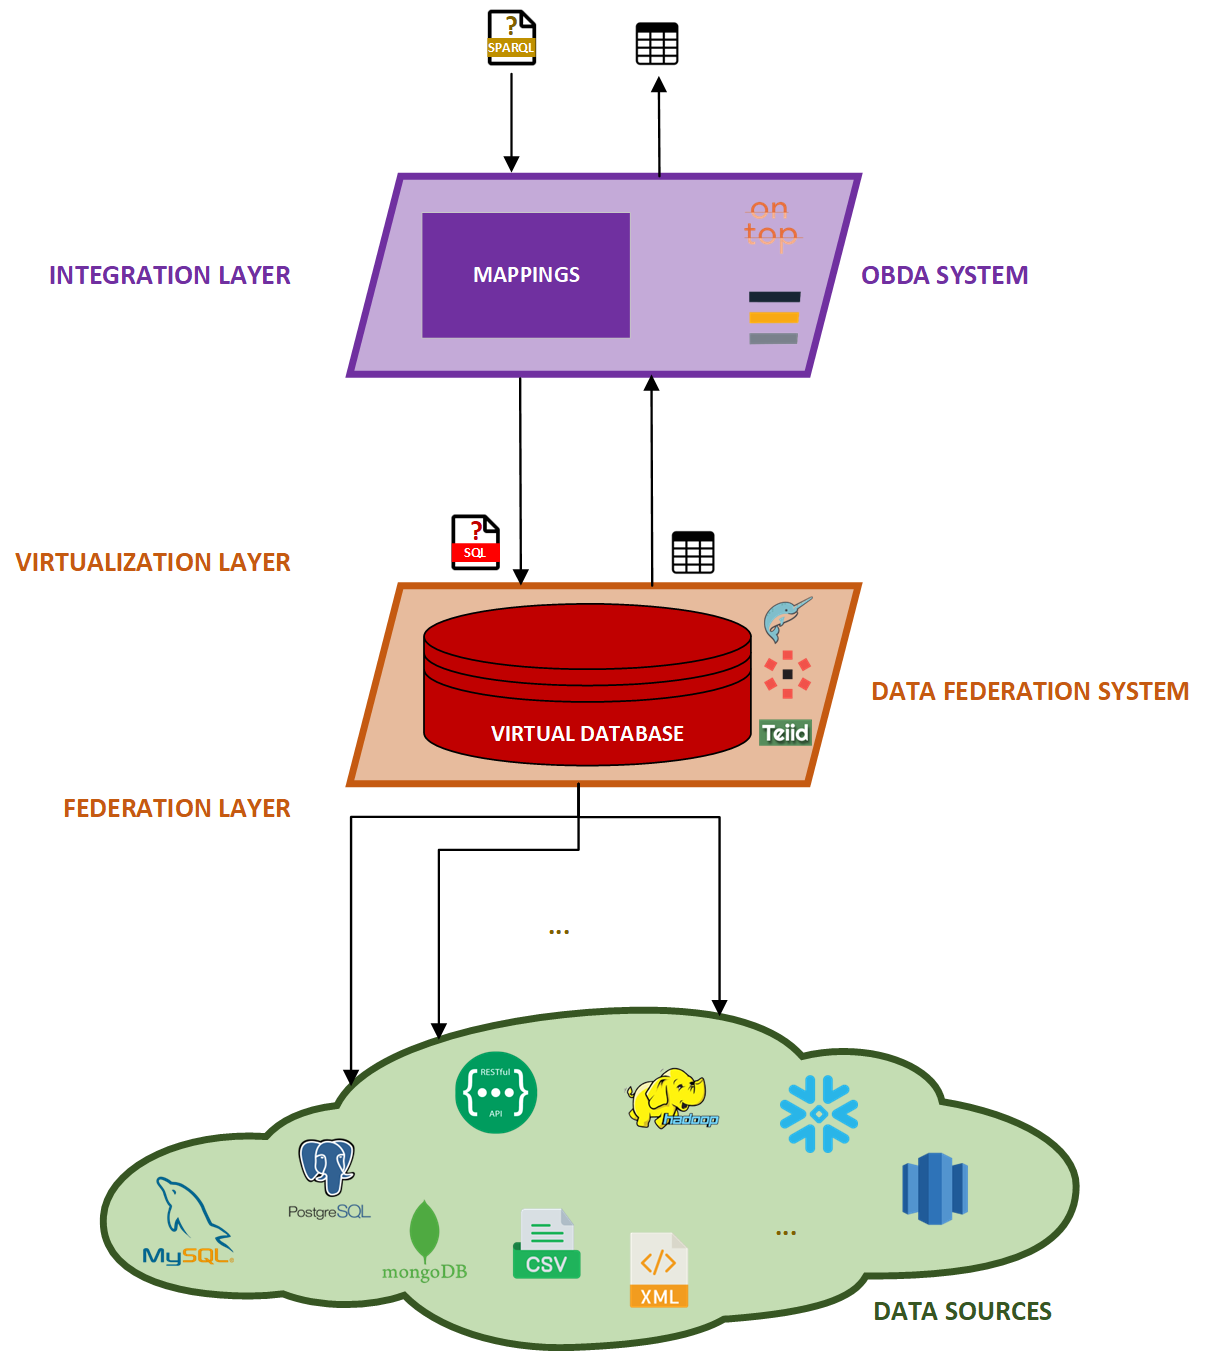
\includegraphics[width=11.5cm]{res/Drawing4.png}
    \caption{OBDF approach}
    \label{fig:obdf}
\end{figure}

Nonetheless, similar design proposal have been implemented in order to address both research questions as well as enterprise requirements. In this section, we will briefly discuss two solutions, one for each environment, analyzing them in details, highlighting strengths and weaknesses.

\section{BigDAWG}
As an example addressing research questions about managing heterogeneous data we have BigDAWG \cite{DBLP:conf/hpec/GadepallyCDEHKM16}, developed under the Intel Science and Technology Center on Big Data. BigDAWG's architecture is composed of four layers: the base layer, the island layer, the main BigDAWG layer, and the application layer. Each layer serves a distinct purpose, from managing diverse physical data stores to facilitating user interaction through applications. This multi-layered approach allows BigDAWG to support various data models and query languages, thus offering a robust solution for cross-database queries and operations.
While traditional systems such as Garlic and IBM DB2 have demonstrated the capability to handle data across different storage systems using a unified interface, BigDAWG distinguishes itself by its comprehensive support for "islands" of different data models. This island approach not only supports operations across various data types but also enhances performance by optimizing queries based on the data model and the underlying database engine. This feature is critical in environments where performance and response times are crucial, such as in medical or real-time analytics applications.
Despite its advanced architecture and capabilities, BigDAWG is not without challenges. It is not available as an off-the-shelf solution; rather, it require certain levels of expertise if someone intends to install it or, in an even worse scenario, there exists the need to develop new islands modules. This means that significant effort would be required to adapt it to specific operational needs. Additionally, there is limited literature and empirical studies on its deployment in real-world scenarios, which poses doubts about considering its implementation.
In summary, while BigDAWG represents a significant advancement in the field of database management systems, its practical application is limited by the prototype nature of its current implementation and the lack of extensive real-world testing. Future research could focus on reducing the barrier to its adoption, refining its architecture based on operational feedback, and expanding its use cases across different scenarios to fully realize its potential.

\section{Optique}
Optique \cite{DBLP:journals/ws/KharlamovMSXKR19}, initially conceived as an EU-funded project under the Seventh Framework Programme \cite{DBLP:journals/ijtm/LytrasSP09}, illustrates a significant advance in the field of \ac{OBDA} tailored for industrial applications. 
This project, which involved multiple institutions including companies like Siemens, aimed to enhance real-time and historical data integration and accessibility using semantic technologies. Unlike typical \ac{OBDA} systems focused predominantly on static data, Optique integrates a robust platform capable of handling both streaming and static data. The project officially ended in 2016.
The Optique platform incorporates a suite of technologies: 
\begin{itemize} 
\item \textbf{STARQL}: An innovative query language that allows complex queries over both streaming and static data, facilitating real-time data processing and analysis;
\item \textbf{ExaStream}: A backend system optimized for low-latency queries, designed to handle high-velocity data streams efficiently;
\item \textbf{OptiqueVQS (Visual Query System)}: A user-friendly component that enhances system accessibility by allowing users to construct queries without prior knowledge of specific query languages, promoting user independence from IT departments. 
\end{itemize}
The project's outcomes are documented extensively, showcasing a scalable approach to data access that significantly reduces reliance on IT intermediation and promotes efficient data utilization \footnote{https://mvnrepository.com/artifact/eu.optique-project}.
Despite its sophisticated capabilities, even if it was conceptualized within an EU-funded project, nowadays Optique is maintained and improved within the Siemens ecosystem, making it de facto a proprietary system. This exclusivity may hinder broader adoption and external validation, potentially impacting its comparative analysis against other \ac{OBDA} systems in diverse real-world settings.
